\documentclass[12pt,letterpaper]{exam}
\usepackage[lmargin=1in,rmargin=1in,tmargin=1in,bmargin=1in]{geometry}
\usepackage{../style/exams}

% -------------------
% Course & Exam Information
% -------------------
\newcommand{\course}{MAT 101: Exam 2}
\newcommand{\term}{Summer -- 2022}
\newcommand{\examdate}{06/02/2022}
\newcommand{\timelimit}{85 Minutes}

\setbool{hideans}{true} % Student: True; Instructor: False

% -------------------
% Content
% -------------------
\begin{document}

\examtitle
\instructions{Write your name on the appropriate line on the exam cover sheet. This exam contains \numpages\ pages (including this cover page) and \numquestions\ questions. Check that you have every page of the exam. Answer the questions in the spaces provided on the question sheets. Be sure to answer every part of each question and show all your work.} 
\scores
%\bottomline
\newpage

% ---------
% Questions
% ---------
\begin{questions}

% Question 1
\newpage
\question[10] Determine whether the relations $f(x)$ and $g(x)$ shown below are functions. If the relation is a function, explain why. If the relation is not a function, explain why not. 
	\[
	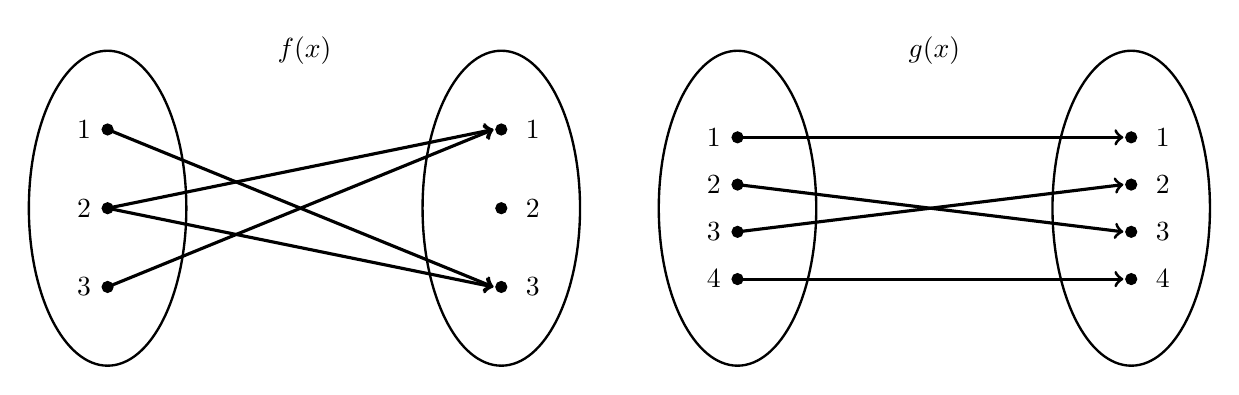
\begin{tikzpicture}
	\node at (2.5,2) {$f(x)$};
	% Ellipses
	\draw[line width=0.03cm] (0,0) circle (1 and 2);
	\draw[line width=0.03cm] (5,0) circle (1 and 2);
	
	% Nodes
	\draw[fill=black] (0,1) circle (0.07);
	\draw[fill=black] (0,0) circle (0.07);
	\draw[fill=black] (0,-1) circle (0.07);
	
	\draw[fill=black] (5,1) circle (0.07);
	\draw[fill=black] (5,0) circle (0.07);
	\draw[fill=black] (5,-1) circle (0.07);
	
	% Arrow
	\draw[line width=0.04cm,->] (0,1) -- (4.9,-1);
	\draw[line width=0.04cm,->] (0,0) -- (4.9,1);
	\draw[line width=0.04cm,->] (0,0) -- (4.9,-1);
	\draw[line width=0.04cm,->] (0,-1) -- (4.9,1);
	
	% Labels
	\node at (-0.3,1) {$1$};
	\node at (-0.3,0) {$2$};
	\node at (-0.3,-1) {$3$};
	
	\node at (5.4,1) {$1$};
	\node at (5.4,0) {$2$};
	\node at (5.4,-1) {$3$};
	
	\tikzset{shift={(8,0)}}
	%
	\node at (2.5,2) {$g(x)$};
	% Ellipses
	\draw[line width=0.03cm] (0,0) circle (1 and 2);
	\draw[line width=0.03cm] (5,0) circle (1 and 2);
	
	% Nodes
	\draw[fill=black] (0,0.9) circle (0.07);
	\draw[fill=black] (0,0.3) circle (0.07);
	\draw[fill=black] (0,-0.3) circle (0.07);
	\draw[fill=black] (0,-0.9) circle (0.07);
	
	\draw[fill=black] (5,0.9) circle (0.07);
	\draw[fill=black] (5,0.3) circle (0.07);
	\draw[fill=black] (5,-0.3) circle (0.07);
	\draw[fill=black] (5,-0.9) circle (0.07);
	
	% Arrow
	\draw[line width=0.04cm,->] (0,0.9) -- (4.9,0.9);
	\draw[line width=0.04cm,->] (0,0.3) -- (4.9,-0.3);
	\draw[line width=0.04cm,->] (0,-0.3) -- (4.9,0.3);
	\draw[line width=0.04cm,->] (0,-0.9) -- (4.9,-0.9);

	
	% Labels
	\node at (-0.3,0.9) {$1$};
	\node at (-0.3,0.3) {$2$};
	\node at (-0.3,-0.3) {$3$};
	\node at (-0.3,-0.9) {$4$};
	
	\node at (5.4,0.9) {$1$};
	\node at (5.4,0.3) {$2$};
	\node at (5.4,-0.3) {$3$};
	\node at (5.4,-0.9) {$4$};
	\end{tikzpicture}
	\]



% Question 2
\newpage
\question[10] Determine whether the relation shown below is a function. If the relation is a function, explain why. If the relation is not a function, explain why not. 
	\[
	\fbox{
	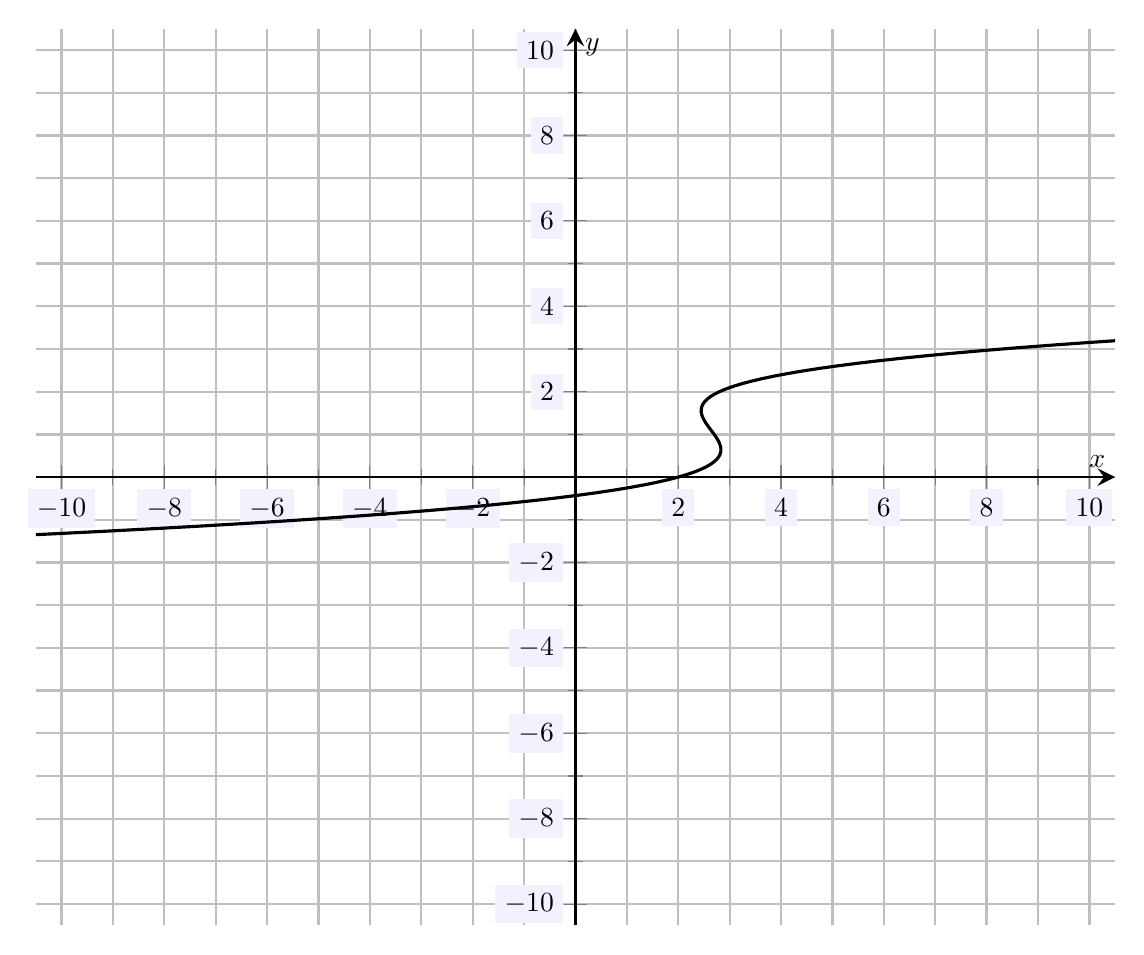
\begin{tikzpicture}[scale=2,every node/.style={scale=0.5}]
	\begin{axis}[
	grid=both,
	axis lines=middle,
	ticklabel style={fill=blue!5!white},
	xmin= -10.5, xmax=10.5,
	ymin= -10.5, ymax=10.5,
	xtick={-10,-8,-6,-4,-2,0,2,4,6,8,10},
	ytick={-10,-8,-6,-4,-2,0,2,4,6,8,10},
	minor tick = {-10,-9,...,10},
	xlabel=\(x\),ylabel=\(y\),
	]
	\addplot[line width= 0.02cm,domain= -2:4, samples=100] ({x^3 - 3.3*x^2 + 3*x + 2},{x}); 
	\end{axis}
	\end{tikzpicture}
	}
	\] 



% Question 3
\newpage
\question[10] For the relation shown below, determine the $x$ and $y$-intercepts. 
	\[
	\fbox{
	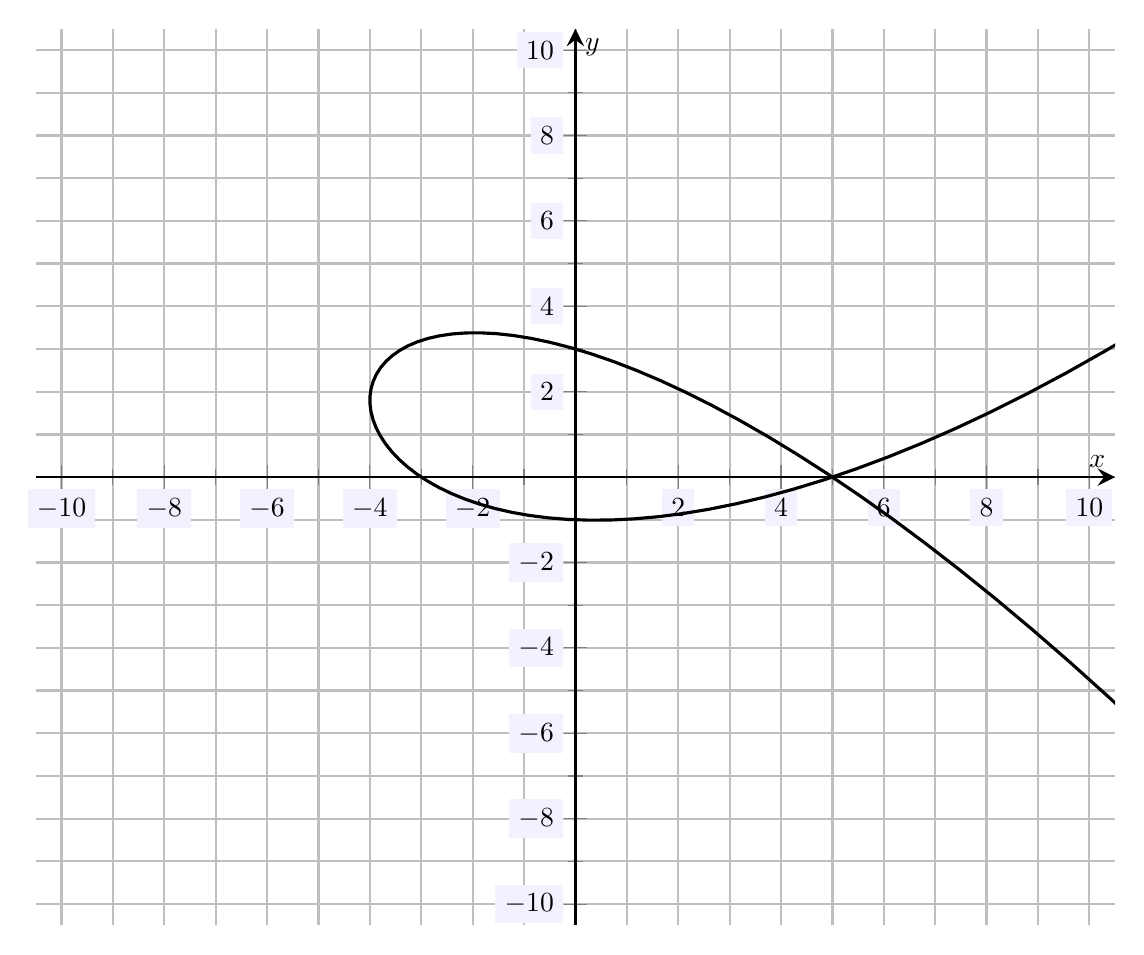
\begin{tikzpicture}[scale=2,every node/.style={scale=0.5}]
	\begin{axis}[
	grid=both,
	axis lines=middle,
	ticklabel style={fill=blue!5!white},
	xmin= -10.5, xmax=10.5,
	ymin= -10.5, ymax=10.5,
	xtick={-10,-8,-6,-4,-2,0,2,4,6,8,10},
	ytick={-10,-8,-6,-4,-2,0,2,4,6,8,10},
	minor tick = {-10,-9,...,10},
	xlabel=\(x\),ylabel=\(y\),
	]
	\addplot[line width= 0.02cm,domain= -10:10, samples=100] ({1/4*(x - 3)*(x + 5)},{1/40*(x - 5)*(x - 1)*(x + 7)}); 
	\end{axis}
	\end{tikzpicture}
	}
	\] 



% Question 4
\newpage
\question[10] Suppose $f(x)$, $g(x)$, and $h(x)$ are functions whose values are given below.
        \begin{table}[!ht]
        \centering
        \begin{tabular}{| c || r | r | r | r | r | r | r |} \hline
	$x$ & $-5$ & $-3$ & $-1$ & $\phantom{-}0$ & $\phantom{-}2$ & $\phantom{-}6$ & $\phantom{-}10$ \\ \hline \hline
	$f(x)$ & $7$ & $10$ & $0$ & $\tfrac{2}{3}$ & $-4$ & $2$ & $\sqrt{2}$ \\ \hline
	$g(x)$ & $0$ & $\pi$ & $6$ & $\tfrac{4}{5}$ & $1$ & $-3$ & $4$ \\ \hline
	$h(x)$ & $\tfrac{9}{8}$ & $0$ & $-3$ & $-1$ & $-1$ & $8$ & $-8$ \\ \hline
        \end{tabular}
        \end{table}

Compute the following, simplifying as much as possible: \pspace
        \begin{enumerate}[(a)]
        \item $(f + h)(-1)=$ \vfill
        \item $(h - f)(10)=$ \vfill
        \item $(-2g)(2)=$ \vfill
        \item $\left( \dfrac{h}{f} \right)(0)=$ \vfill
        \item $g(-3)\, h(6)=$ \vfill
        \item $h(2 - f(2))=$ \vfill
        \item $(g \circ h)(0)=$ \vfill
	\item $(f \circ g)(-5)=$ \vfill
        \item $(g \circ f)(6)=$ \vfill
	\item $(g \circ f \circ h)(-1)=$ \vfill
        \end{enumerate} 



% Question 5
\newpage
\question[10] Suppose $f(x)$ and $g(x)$ are the functions given below. 
	\[
	\begin{aligned}
	f(x)&= 1 - x^2 \\[0.3cm]
	g(x)&= 2x + 1
	\end{aligned}
	\]

Compute the following, simplifying as much as possible: \pspace
        \begin{enumerate}[(a)]
	\item $\left( \dfrac{f}{g} \right)(x)=$ \vfill
        \item $g(x) - f(x)=$ \vfill
        \item $f(x) \, g(x)=$ \vfill
        \item $(f \circ g)(x)=$ \vfill
        \item $(g \circ f)(x)=$ \vfill
        \end{enumerate} 



% Question 6
\newpage
\question[10] Suppose that $f(x)$ is a function defined on all real numbers whose inverse exists. A few values of $f(x)$ are given below.
        \begin{table}[!ht]
        \centering
        \begin{tabular}{c || r | r | r | r} 
	$x$ & $1$ & $2$ & $3$ & $4$ \\ \hline
	$f(x)$ & $3$ & $4$ & $1$ & $2$
        \end{tabular}
        \end{table}

Compute the following: \pspace
	\begin{enumerate}[(a)]
	\item $f(4)=$ \vfill
	\item $\big( f(1) \big)^2=$ \vfill
	\item $f^{-1}(3)=$ \vfill
	\item $f^{-1}(f(20))=$ \vfill
	\item $(f \circ f^{-1})(5)=$ \vfill
	\end{enumerate}



% Question 7
\newpage
\question[10] Explain whether the relation shown below has an inverse. If it does, sketch the inverse. If it does not, explain why. 
	\[
	\fbox{
	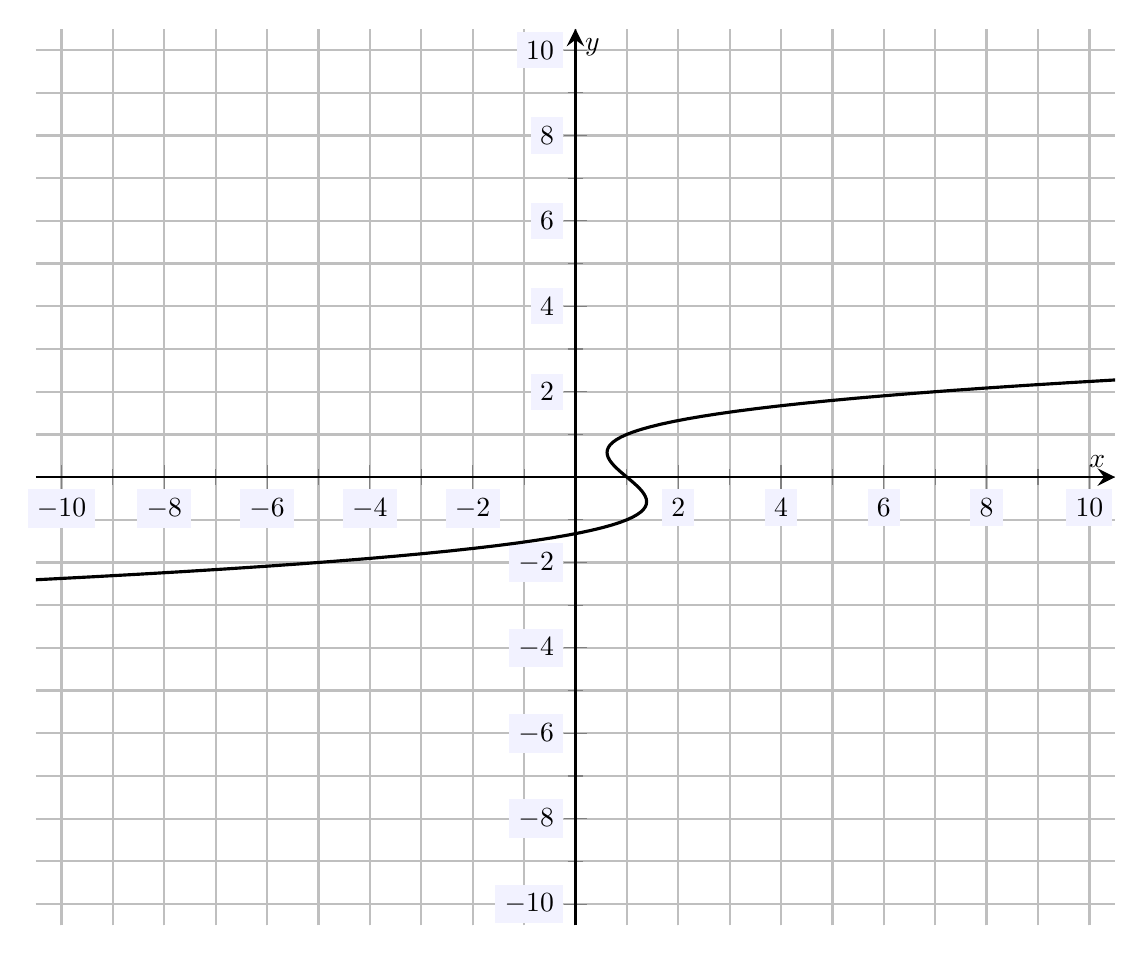
\begin{tikzpicture}[scale=2,every node/.style={scale=0.5}]
	\begin{axis}[
	grid=both,
	axis lines=middle,
	ticklabel style={fill=blue!5!white},
	xmin= -10.5, xmax=10.5,
	ymin= -10.5, ymax=10.5,
	xtick={-10,-8,-6,-4,-2,0,2,4,6,8,10},
	ytick={-10,-8,-6,-4,-2,0,2,4,6,8,10},
	minor tick = {-10,-9,...,10},
	xlabel=\(x\),ylabel=\(y\),
	]
	\addplot[line width= 0.02cm,domain= -3:3, samples=100] ({x^3 - x +1},{x});
	\end{axis}
	\end{tikzpicture}
	}
	\] 



% Question 8
\newpage
\question[10] As accurately as possible, sketch the line $2x - 3y= 6$ on the plot below. Your plot should include at least three points that are exactly on the line. 
	\[
	\fbox{
	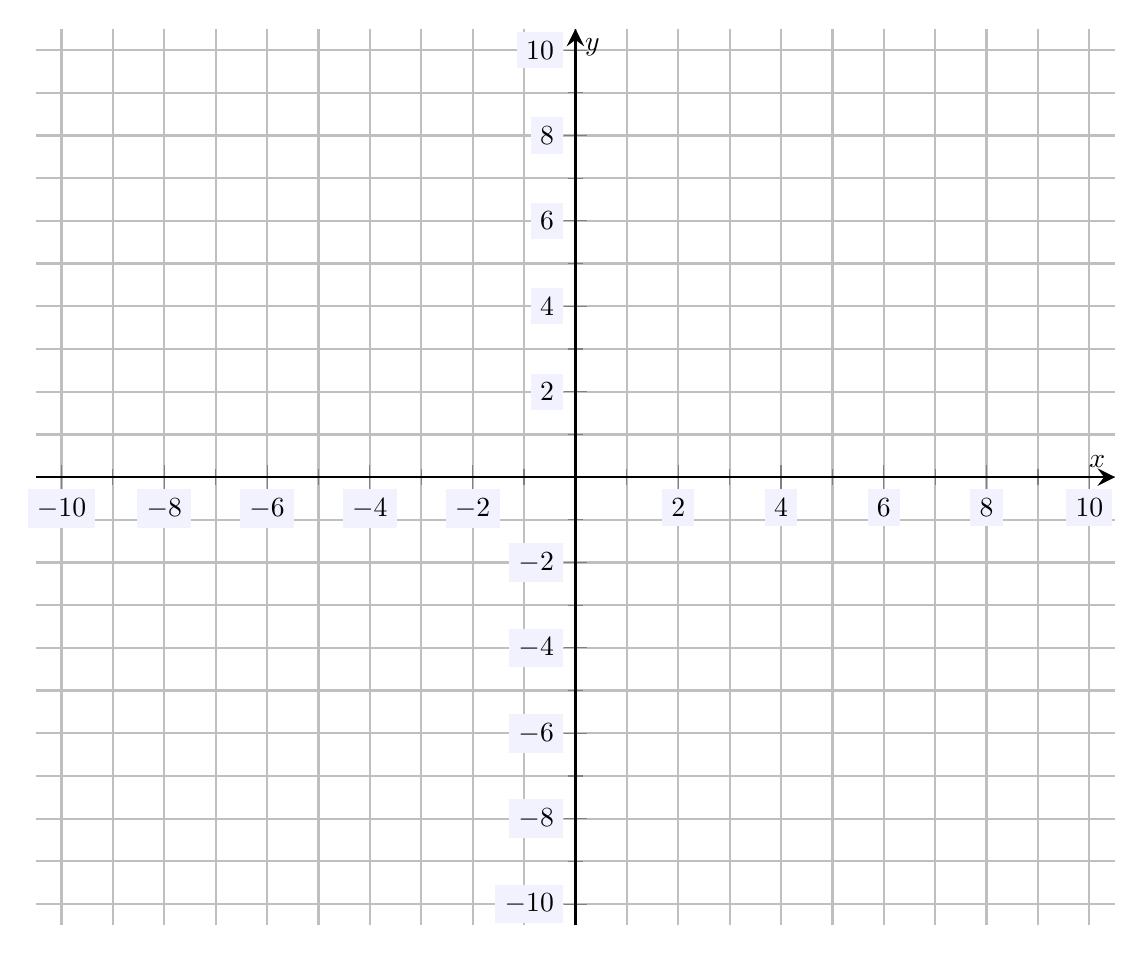
\begin{tikzpicture}[scale=2,every node/.style={scale=0.5}]
	\begin{axis}[
	grid=both,
	axis lines=middle,
	ticklabel style={fill=blue!5!white},
	xmin= -10.5, xmax=10.5,
	ymin= -10.5, ymax=10.5,
	xtick={-10,-8,-6,-4,-2,0,2,4,6,8,10},
	ytick={-10,-8,-6,-4,-2,0,2,4,6,8,10},
	minor tick = {-10,-9,...,10},
	xlabel=\(x\),ylabel=\(y\),
	]
	\end{axis}
	\end{tikzpicture}
	}
	\] 



% Question 9
\newpage
\question[10] Determine whether the table of values below could be given by a linear function. If not, explain why. If it can, find the linear function.
        \begin{table}[!ht]
        \centering
        \begin{tabular}{|c || r | r | r |} \hline
	$x$ & $0.2$ & $3.6$ & $5.1$ \\ \hline
	$y$ & $9.84$ & $-1.38$ & $-6.33$ \\ \hline
        \end{tabular}
        \end{table}



% Question 10
\newpage
\question[10] Determine whether the following lines are the parallel, perpendicular, or neither. Be sure to justify your answer. 
	\[
	\begin{aligned}
	\ell_1 &\colon & 2x - y&= 5 \\[0.3cm]
	\ell_2 &\colon & -2x + 4y&= 24
	\end{aligned}
	\] 



% Question 11
\newpage
\question[10] Consider the line $4x - 6y= 12$.
	\begin{enumerate}[(a)]
	\item Determine the slope of the given line.
	\item Interpret the slope in at least two different ways.
	\item Is the function whose graph is the given line an increasing or decreasing function? Explain. 
	\item Determine the $y$-intercept of the given line. 
	\item Determine the $x$-intercept of the given line. 
	\end{enumerate}



% Question 12
\newpage
\question[10] A caterer charges a flat fee for each person for whom a meal has to be prepared. The caterer charges \$270 for 15 people and \$360 for 20 people. Let $C(p)$ denote the cost of hiring the caterer to prepare food for $p$ people. 
	\begin{enumerate}[(a)]
	\item Explain why $C(p)$ is linear.
	\item Find $C(p)$.
	\item Interpret the slope of $C(p)$ in the context of the problem. 
	\item Find and interpret $C(32)$. 
	\end{enumerate}



% Question 13
\newpage
\question[10] A certain species of fungus reproduces by releasing tiny spores. The larger the fungus, the more spores that are released. Scientist find that the number of spores (in thousands) a fungus with diameter $d$ (in inches) can be modeled by $N(d)= -3.5 + 15.5d$.
	\begin{enumerate}[(a)]
	\item Find and interpret the slope of $N(d)$ in the context of the problem.
	\item Find and interpret in the context of the problem, if possible, the $y$-intercept of $N(d)$.
	\item According to the model, how large would the fungus have to be in order for it to release 100,000 spores?
	\end{enumerate}



% Question 14
\newpage
\question[10] Showing all your work, find the equation of the line whose $x$-intercept is $(-1, 0)$ that has slope $-\frac{6}{7}$. 



% Question 15
\newpage
\question[10] Showing all your work, find the equation of the line that is parallel to the line $x= 4$ that contains the $y$-intercept of the line $-6x + 5y= 11$. 



% Question 16
\newpage
\question[10] Showing all your work, find the equation of the line that is perpendicular to the line $y= 6 - 7x$ at its $y$-intercept. 



% Question 17
\newpage
\question[10] Showing all your work, solve the following equation and then verify your solution:
	\[
	6 \left( \dfrac{1}{2}\,x + 5 \right)= 28
	\]



% Question 18
\newpage
\question[10] Showing all your work, solve the following equation:
	\[
	7x + 4= 6 - 2(3 - x)
	\]



% Question 19
\newpage
\question[10] Showing all your work, solve the following equation:
	\[
	\sqrt{2} \left( x - \sqrt{2} \right)= \dfrac{x + 5}{3}
	\]



% Question 20
\newpage
\question[10] Showing all your work, solve the following equation:
	\[
	\dfrac{x + 6}{1 - x}= 10
	\]


\end{questions}
\end{document}